\documentclass{article}


\usepackage[]{algorithm2e}

\usepackage{fullpage}
\usepackage{color}
\usepackage{amsmath}
\usepackage{url}
\usepackage{verbatim}
\usepackage{graphicx}
\usepackage[export]{adjustbox}
\usepackage{parskip}
\usepackage{amssymb}
\usepackage{listings} 


% Colors
\definecolor{blu}{rgb}{0,0,1}
\def\blu#1{{\color{blu}#1}}
\definecolor{gre}{rgb}{0,.5,0}
\def\gre#1{{\color{gre}#1}}
\definecolor{red}{rgb}{1,0,0}
\def\red#1{{\color{red}#1}}

% Math
\def\norm#1{\|#1\|}
\def\R{\mathbb{R}}
\def\argmax{\mathop{\rm arg\,max}}
\def\argmin{\mathop{\rm arg\,min}}
\newcommand{\mat}[1]{\begin{bmatrix}#1\end{bmatrix}}
\newcommand{\alignStar}[1]{\begin{align*}#1\end{align*}}

% LaTeX
\newcommand{\fig}[2]{\includegraphics[width=#1\textwidth]{#2}}
\newcommand{\centerfig}[2]{\begin{center}\includegraphics[width=#1\textwidth]{#2}\end{center}}
\def\items#1{\begin{itemize}#1\end{itemize}}
\def\enum#1{\begin{enumerate}#1\end{enumerate}}

\begin{document}

\title{CPSC 340 Assignment 1 (due 2018-01-17 at 9:00pm)}
\author{Henry Deng \\ Student Number: 41584103}
\date{}
\maketitle

\vspace{-4em}

\section{Data Exploration}

\subsection{Summary Statistics}
The minimum, maximum, mean, median, and mode of all values across the dataset.
\\ \blu{minimum}: 0.3520
\\ \blu{maximum}: 4.8620
\\ \blu{mean}: 1.3246
\\ \blu{median}: 1.1590
\\ \blu{mode}: 0.7700
\enum{
\item The $5\%$, $25\%$, $50\%$, $75\%$, and $95\%$ quantiles of all values across the dataset.
\\ $5\%$: 0.465
\\ $25\%$: 0.718
\\ $50\%$: 1.159
\\ $75\%$: 1.813
\\ $95\%$: 2.624
\item The names of the regions with the highest and lowest means, and the highest and lowest variances.
\\ highest mean: WtdILI
\\ lowest mean: Pac 
\\ highest variance: Mtn 
\\ lowest variance: Pac 
}

The mode is not a reliable estimate because we are working with continuous data. Instead, looking at the interquantile range is a more reliable measurement.  

\subsection{Data Visualization}

The figure contains the following plots, in a shuffled order:
\enum{
\item A single histogram showing the distribution of \emph{each} column in $X$.
\\ Plot \textbf{C}. \blu{Reason:} C is a histogram and displays less columns than D 
\item A histogram showing the distribution of each the values in the matrix $X$.
\\ Plot \textbf{D}. \blu{Reason:} D is a histogram and displays more values (since it's in the matrix) than C does.
\item A boxplot grouping data by weeks, showing the distribution across regions for each week.
\\ Plot \textbf{B}. \blu{Reason:} B is the only boxplot out of all the plots and unlike A, it shows the distribution across the regions for each week.
\item A plot showing the illness percentages over time.
\\ Plot \textbf{A}. \blu{Reason:} A shows the illness percentage for each region over time. 
\item A scatterplot between the two regions with highest correlation.
\\ Plot \textbf{F}. \blu{Reason:} F is a scatterplot but unlike E, the points are closer to each other and form more of a linear relationship, which means the correlation is higher. 
\item A scatterplot between the two regions with lowest correlation.
\\ Plot \textbf{E}. \blu{Reason:} E is a scatterplot but unlike F, the points are further apart from each other so there is less correlation. 
}

\section{Decision Trees}

\subsection{Splitting rule}

Yes. For categorical features, equality splitting can be appropriate.

\subsection{Decision Stump Implementation}
\begin{verbatim}
Refer to: https://github.ugrad.cs.ubc.ca/CPSC340-2017W-T2/c1z8_a1/blob/master/code/decision_stump.py
\end{verbatim}
Updated error: \blu{0.253}

\subsection{Constructing Decision Trees}
\begin{verbatim}
Refer to: https://github.ugrad.cs.ubc.ca/CPSC340-2017W-T2/c1z8_a1/blob/master/code/simple_decision.py
\end{verbatim}

\subsection{Decision Tree Training Error}

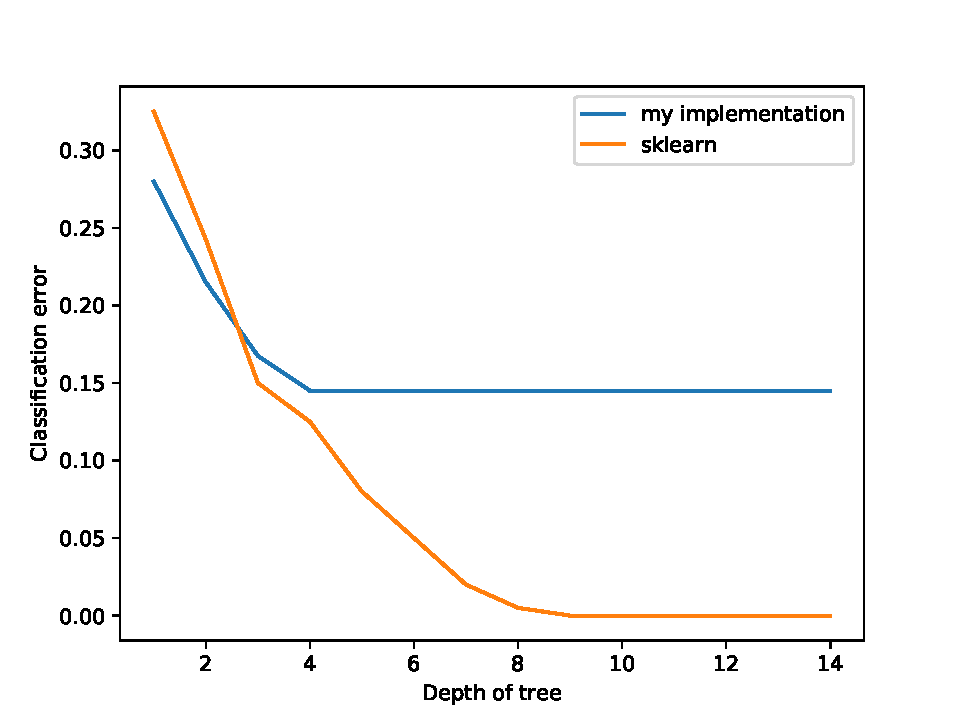
\includegraphics[scale=0.8]{../figs/q2_4_tree_errors}
\\ \centerline{Fig 1. Classification error vs. Depth}

One major difference is that the training error in the scikit-learn version gradually goes down to 0. However, our training error cannot reach 0 because at a certain point, the computed error is not lower than the current minimum error as highlighted by this line:
\begin{verbatim}
if errors < minError:
// do something
\end{verbatim}

\subsection{Cost of Fitting Decision Trees}

The total cost is O($mndlogn$), which takes in account sorting and going through each depth, up to a depth of m. 

\section{Training and Testing}

\subsection{Training and Testing Error Curves}

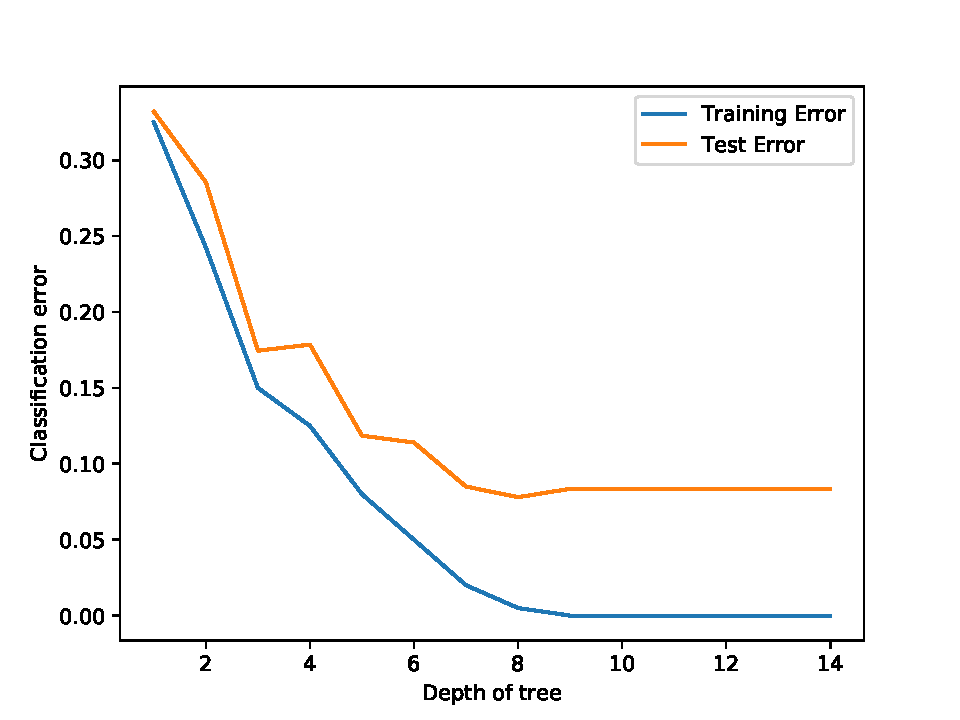
\includegraphics[scale=0.8]{../figs/q3_1_train_vs_test}
\\ \centerline{Fig 2. Training and Testing Error vs. Depth}

Both test and training error goes down; however, training error goes down to 0 but test error plateaus around depth 8.
 
\subsection{Validation Set}

If we use the first half samples to train and the second half to validate, the depth to minimize validation set error is around 3. However, if we switch the training and validation set data, the depth to minimize validation set error is around 6. In order to use more of our data, we could cross-validate. 

\section{K-Nearest Neighbours}

\subsection{KNN Prediction}

\hspace{3mm} 1. The predict function is implemented at
\begin{verbatim} 
https://github.ugrad.cs.ubc.ca/CPSC340-2017W-T2/c1z8_a1/blob/master/code/knn.py
\end{verbatim}
\enum{
\item[2.] When k = 1, the training error is 0 and test error is 0.065
\\ When k = 3, the training error is 0.028 and test error is 0.066
\\ When k = 10, the training error is 0.072 and the test error is 0.097
\item[3.] Plot generated by utils.plotClassifier \\
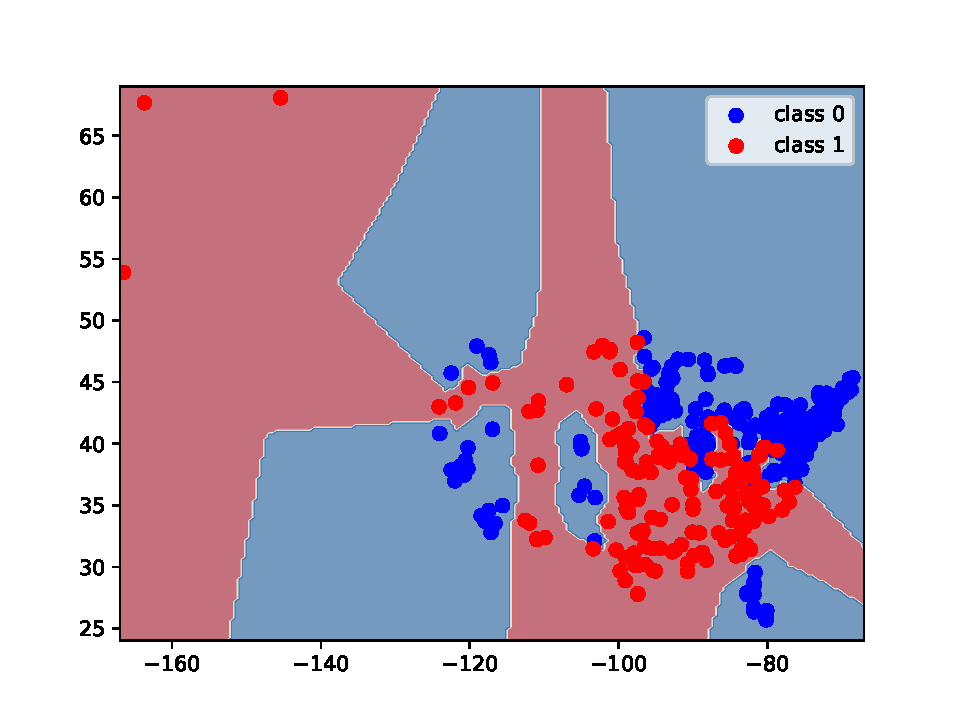
\includegraphics[scale=0.8]{../figs/q4_1_knn_plot_classifier}
\\ \centerline{Fig 3. KNN plot generated by utils.plotClassifier on the citiesSmall dataset for k = 1}
\item[4.] This is because each data is a nearest neighbour of itself when k = 1. Therefore, yhat is calculated based on y's value. Since yhat = y, the training error must be 0. 
\item[5.] Using a similar method as before, we could use cross-validation on our training and validation set to determine the value of k that minimizes validation error.
}
\subsection{Condensed Nearest Neighbours}

\enum{
\item The CNN algorithm took around 4.3s to run for k = 1, whereas the KNN algorithm took way longer (stopped running it after 15s)
\item Training error = 0.0075, test error = 0.0176, variables = 457
\item Plot generated by utils.plotClassifier \\
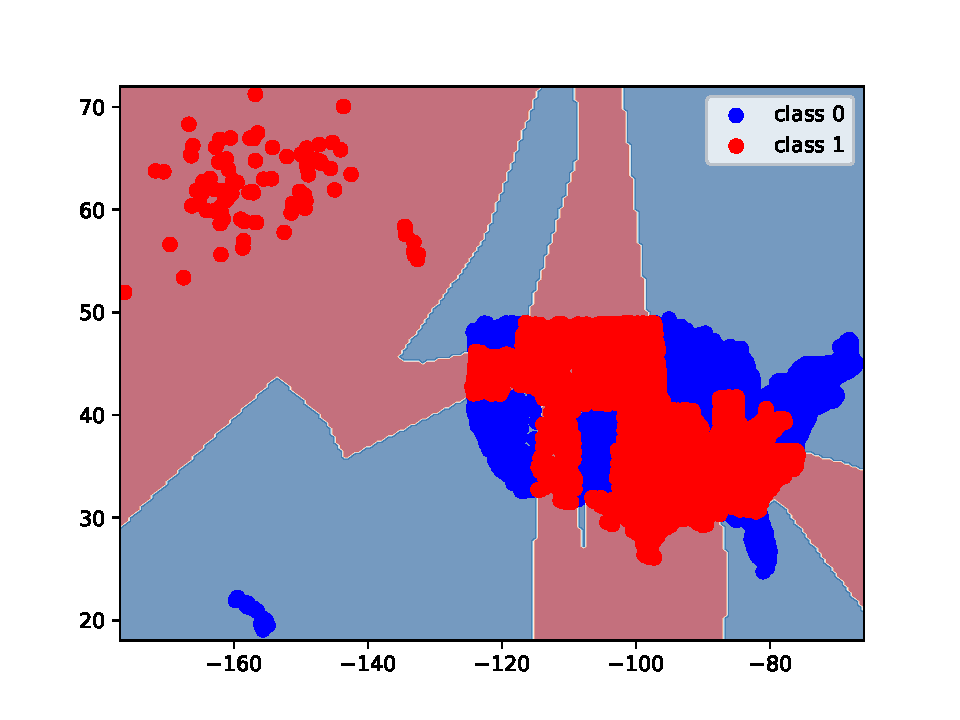
\includegraphics[scale=0.8]{../figs/q4_2_cnn_plot_classifier}
\\ \centerline{Fig 4. CNN plot generated by utils.plotClassifier on the citiesBig1 dataset for k = 1}
\item Since only a subset of the training example is stored, the nearest one neighbour is no longer itself. If a data point is not included in the training subset, then it cannot be a neighbour of itself -- therefore, yhat != y, and the training error is not 0. 
\item The run time is O($tds$)  
\item The test error is high because we are violating the assumption that the samples are identically and independently distributed (IID) because the training set as well as the testing set are grouped by states. The training error is high because it is difficult to correctly classify every object, which results in underfitting in the model.  
\item The decision tree model ran faster than CNN. I personally prefer the decision tree model for this dataset. \\
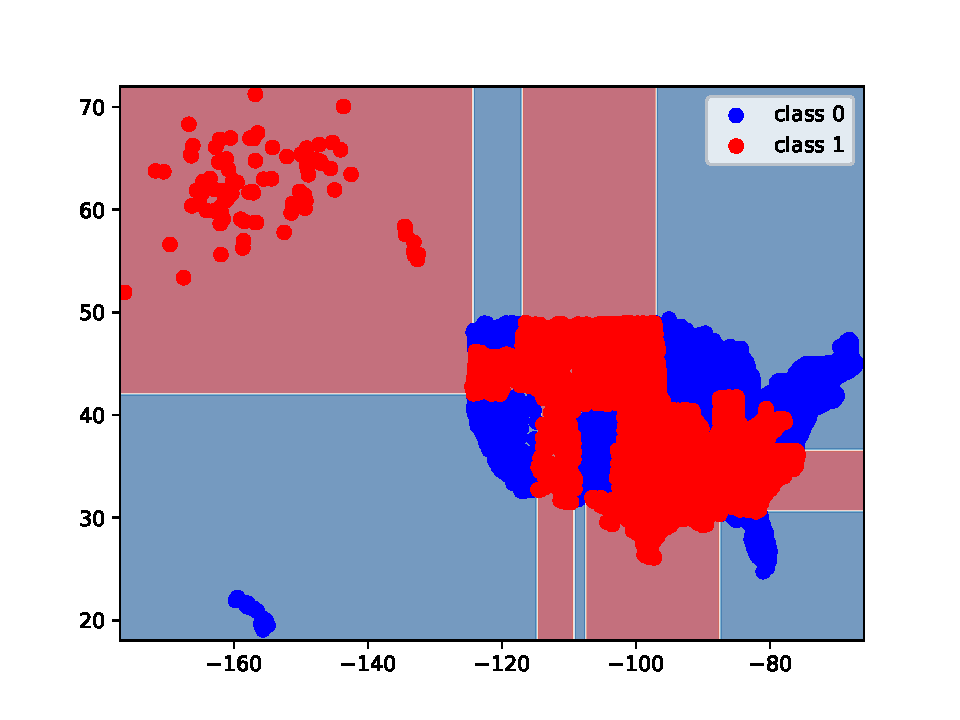
\includegraphics[scale=0.8]{../figs/q4_2_decision_plot_classifier}
\\ \centerline{Fig 5. Decision tree plot generated by utils.plotClassifier on the citiesBig1 dataset with default hyperparameters}
}

\section{Very-Short Answer Questions}

\enum{
\item Looking at the scatterplot tells us the distribution of the data, which is useful for choosing which models to use for our data. 
\item If all objects do not come from the same distribution (such as the food allergy example in class), then we have data that depend on each other -- which violates IDD. 
\item Validation set is used during training and is used to determine whether you're overfitting or underfitting your data. The test set cannot be used to train the model but it is used to evaluate how well the model does with data that is outside the training set.  
\item Non-parametric models allow for more complex models with large datasets because the number of parameter grows with 'n' whereas parametric models have a fixed number of parameters, which means it doesn't scale well with data. 
\item Standardization doesn't change the accuracy of a decision tree model. Standardization does increase the accuracy of KNN, especially if we have numerical variables.
\item Increasing k does not affect the prediction runtime because predictions take O($tnd$) time where O($nd$) is the cost of predicting 1 test object, multiplied by $t$ test objects. Increasing k also doesn't increase the training runtime because KNN has no training phase (since it is a lazy model). 
\item When k = 1, there is no training error, but as k increases, the training error goes up as k increases. The test error decreases initially and then goes up as k increases.
\item For parametric models, training error decreases to 0 as the data size increases (due to overfitting). Test error decreases initially and then increases as data size increases. 
}

\end{document}
